\documentclass[conference]{IEEEtran}
%\IEEEoverridecommandlockouts
% The preceding line is only needed to identify funding in the first footnote. If that is unneeded, please comment it out.
\usepackage{cite}
\usepackage{amsmath,amssymb,amsfonts}
\usepackage{algorithmic}
\usepackage{graphicx}
\usepackage{textcomp}
\usepackage{xcolor}
\def\BibTeX{{\rm B\kern-.05em{\sc i\kern-.025em b}\kern-.08em
    T\kern-.1667em\lower.7ex\hbox{E}\kern-.125emX}}
\begin{document}

\title{Evolving Music with Genetic Algorithm%\\
%{\footnotesize \textsuperscript{*}Note: Sub-titles are not captured in Xplore and
%should not be used}
%\thanks{Identify applicable funding agency here. If none, delete this.}
}

\author{\IEEEauthorblockN{Nisha Shareef Shaikh}
\IEEEauthorblockA{\textit{BSc. Computer Science} \\
\textit{Class of 2020}\\
\textit{Habib University}\\
Karachi, Pakistan \\
ns02530@st.habib.edu.pk}
\and
\IEEEauthorblockN{Abeera Tariq}
\IEEEauthorblockA{\textit{BSc. Computer Science} \\
\textit{Class of 2020}\\
\textit{Habib University}\\
Karachi, Pakistan \\
at02787@st.habib.edu.pk}
}

\maketitle

\begin{abstract}
%This paper has been generated as a report for a project in the course, Computational Intelligence. Using skills learned in this course, we have aimed to approach a novel scheme to produce music.
This paper aims to use a genetic algorithm to produce music. This approach involves constructing melodies from random notes and pitches and evolving them to create a pleasant composition.
\end{abstract}

\begin{IEEEkeywords}
music, evolution, genetic algorithm
\end{IEEEkeywords}

\section{Introduction}
%Motivation, Novelty, How your paper is tackling it and what it does well
Algorithms in music are used for sound synthesis, sampling, recognition of musical works and for music composition. Music composition involves innovation, creativity and a sense of melody. Through this project, we hope to discover how music can be composed without the involvement of musicians. Taking motivation from \cite{b1}, we will try to utilize our knowledge of genetic algorithms to compose melodies.

Composing music is thought to be a process that can't work without human involvement due to the subjective nature of the task as an artist composes music as a means to express their feelings, emotions and inspiration. It is believed that music is composed as a result of free choice of existing rules. This implies that the process of composition can be broken down to a set of instructions, so composition may be considered an algorithm in some way. Since genetic algorithms are capable of mimicking  nature, they are believed to be a suitable approach to eliminate human involvement. However, the lack of human factor may lead to large amounts of objectively bad and useless music.

With the genetic algorithm we implemented, melodies will be represented as a list of integers that describe each beat's note, octave and duration. The algorithm will start with a group of random compositions created with random parameters to describe each beat. This group will be evolved with the algorithm to continuously improve the compositions and get a pleasant-sounding piece at the end.

\section{Technical Background}
%Explain techniques used in the project
The main technique used in this paper is the genetic algorithm. It has been inspired by the process of biological evolution and proves beneficial for optimization. Using concepts of reproduction, mutation, selection and recombination on candidate solutions (chromosomes), genetic algorithms can solve an optimization problem. A fitness function determines how good the candidate solution is and works by evolving the solutions to obtain the optimum solution to the problem.

The algorithm starts by generating a population with $n$ chromosomes, where $n$ is determined by the user and every chromosome denotes a candidate solution to the problem.

From this population, certain chromosomes are selected for reproduction on the basis of their fitness value (depending on the selection scheme used). For reproduction, a crossover method is used where a crossover point is selected, the two parents selected are split at this crossover point, and a new solution or offspring is created by joining the head of one parent with the tail of the other. Once the offspring have been generated and added to the population, they will be mutated with a certain probability. For mutation, a certain gene of the chromosome will be changed. The population will again be reduced to just $n$ solutions by selecting the best $n$ chromosomes from the current population.

This process of reproduction, mutation and selection will keep repeating until the criteria of termination have been fulfilled.

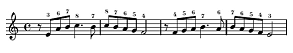
\includegraphics{music.png}\\

Before we proceed, it is important to understand some terms in music.

\subsection{Note}
A note is the pitch (frequency) and duration of a sound generally represented by letters,
\begin{center}
    $C-D-E-F-G-A-B$
\end{center}
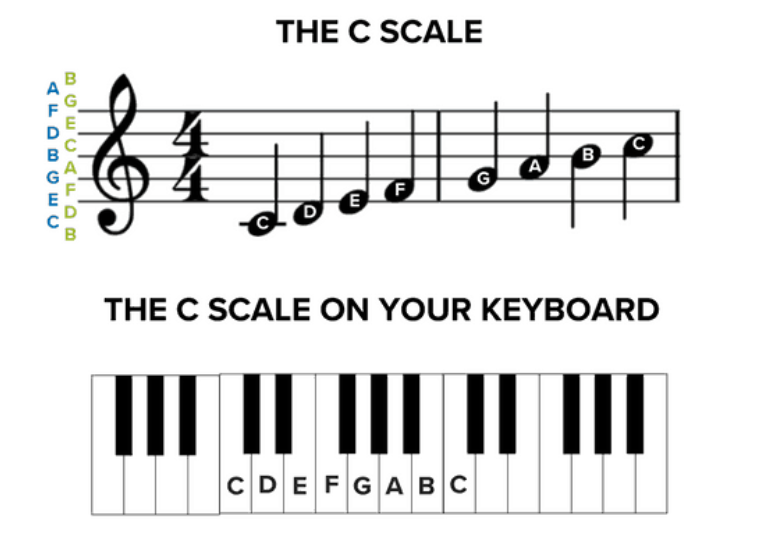
\includegraphics[width=7 cm, height=7 cm]{notes.png}

\subsection{Octave}
Octave is a series of eight notes, where 2 notes are separated by intervals. Consecutive octaves have half or twice the frequency of each other.

\subsection{Bar}
The duration of the tone and frequency of the durations in the melody defines rhythm and basic unit of measurement - bar. It organizes the written music in small sections where each bar is a section of time and usually contains the same number of beats in it.



\section{Related Work}
%How other people have done it, What problems they faced
The inspiration to our study is \textit{"A Genetic Algorithm For Composing Music" by Dragan Matic} \cite{b1} which exposed us to intelligent music composition for the first time. The paper elaborates on composing melodies based on a reference melody. With a different mechanism involved for constructing a melody, the idea of composition in this paper is restricted to a similarity value of a chromosome with respect to a reference melody. The similarity is calculated based on a defined \textit{``distance"} of an individual with the reference one.

The implementation of genetic algorithm is based on simply \textit{mutation} where each generation is only mutated to evolve and compose better pieces of music. The algorithm utilizes 3 different ways to mutate the chromosomes. An interesting mechanism of selection is utilized called \textit{elimination selection} whereby all individuals of low fitness are removed and all duplicates (individuals of the same fitness) are also removed. Therefore, at each iteration, the population consists of individuals with distinct fitness. Experimentation and results of this study proved fruitful as it resulted in a beautiful composition as claimed by the researcher. Although the algorithm leaves possible room for controlling parameters, the existence of a reference melody assists in producing more rhythmic and harmonious music. The algorithm is designed in such a way so as to incorporate mathematical functions that evaluate fitness based on other parameters.

Gaining inspiration from this algorithm, we have attempted to use some mathematical functions to determine fitness of the melodies which will be discussed ahead in this paper.

\section{Methodology}
Our approach is to utilize our learning of genetic algorithm to compose music. We start by randomly generating notes to create random melodies, which will comprise our population. These melodies will then go through the reproduction, mutation and selection processes for a certain number of generations.

\subsection{Chromosome Structure}
The chromosome for a melody is represented as a list of 4-tuples, where each tuple defines a single beat. For example, a beat may be represented as $(0, 4, 32, 4)$, where each index is defined as follows
\begin{itemize}
	\item Index 0: Note Index
	\item Index 1: Octave Index
	\item Index 2: Absolute Note
	\item Index 3: Duration
\end{itemize}

The note index will refer to the notes $C, D, E, F, G, A,$ and $B$ along with rest (which, in music terminology, means an interval of silence). Hence, in the example above, the beat is a $C$ note.

Octave is basically the interval between two notes with the same letter name with one having double or half the frequency of the other. For example, the octave can go from $C-C$ with one $C$ note having half or double the frequency of the other $C$ note. Hence, the beat above is a $C4$ note.

The absolute note represents the note and octave together as one integer to facilitate in the functioning of the genetic algorithm. It is basically the product of the octave index and the number of notes per octave added to the letter index.

The duration specifies the amount of time that the beat would play for. The duration $d$ is a denominator in the fraction $\frac{1}{d}$, so in the example above, the beat will play for one-fourth or a quarter of a second. If the duration was 2, the beat would play for half a second.

\begin{center}
    [(0, 4, 32, 4), (6, 0, 6, 4), (4, 2, 20, 4), (6, 1, 14, 4),\\ (2, 1, 10, 4), (3, 1, 11, 4), (1, 3, 25, 4), (3, 4, 35, 4),\\ (5, 0, 5, 4), (0, 2, 16, 4), (7, 3, 31, 4), (2, 5, 42, 4),\\ (5, 3, 29, 4), (0, 2, 16, 4), (1, 5, 41, 4), (6, 0, 6, 4),\\ (7, 3, 31, 4), (7, 5, 47, 4), (5, 0, 5, 4), (0, 3, 24, 4),\\ (2, 3, 26, 4), (0, 5, 40, 4), (2, 5, 42, 4), (0, 1, 8, 4),\\ (3, 5, 43, 4), (4, 4, 36, 4), (5, 3, 29, 4), (5, 5, 45, 4),\\ (1, 1, 9, 4), (7, 3, 31, 4), (7, 4, 39, 4), (1, 1, 9, 4)]\\
    
    Representation of a single melody as a chromosome
\end{center}

\subsection{Selection Schemes}
Selection schemes are applied to choose the fittest parents and find the best solutions to survive in the next generation. The selection schemes used include binary tournament and truncation.

%\textit{1. Binary Tournament}
\subsubsection{Binary Tournament}
Binary tournament involves randomly selecting two chromosomes and choosing the fittest of the two according to a pre-determined selection probability. A random number is generated and if the number is lower than or equal to the selection probability, the fitter individual is chosen or else the weaker one is chosen. The binary tournament process is run for as many times as the number of chromosomes to be selected.

%\textit{2. Truncation}
\subsubsection{Truncation}
Truncation selection chooses the top $k$ fittest chromosomes, where $k$ is the number of chromosomes that have to be selected. For each crossover, 2 fittest chromosomes are selected, while for survivor selection, $k$ is equal to the population size to select chromosomes that will be carried over to the next generation.

\subsection{Fitness Function}
The fitness is evaluated based on several weighted attributes of music. The general formula for evaluating the fitness $f$ is
\begin{align*}
f &= \sum_{i=1}^{n} \lambda_{i}f_{i}
\end{align*}
where $f_{i}$ is the musical attribute being used, $\lambda_{i}$ is the weight of the attribute and $n$ is the total number of attributes used.

Following are the attributes we used:

\subsubsection{Octave}
A composition sounds more pleasant if the pitch values of its notes are relatively close to each other \cite{b2}. Pitch and octave are similar in that they both denote the frequency of the note. Hence, to make sure the pitches are close to each other, we favored chromosomes that have more beats with the same octave.

\subsubsection{Interval}
As the compositions have been created randomly, there is a chance that large intervals might occur, which do not sound too pleasing \cite{b3}. Hence, this function would give better fitness scores to compositions with small intervals. The perfect fourth interval is preferred \cite{b1} because it sounds the most pleasing to the ears.

\subsubsection{Variation}
This function evaluates the amount of changes in pitch direction \cite{b2}. Frequent variation in pitch direction does not sound aesthetically pleasing to the ears, so this function rewards compositions with a more stable direction. The function will evaluate every three succeeding notes to see if they all rise or fall, awarding better scores if all three are in the same direction.

\subsubsection{Down Beat}
Down beat is the first beat in a bar and is usually the most significant one. Chord notes (which are $C, E$ and $G$ in our case) sound better as the down beat, so compositions with a higher number of bars with a chord note as the down beat will be given a better fitness score.

\begin{figure}
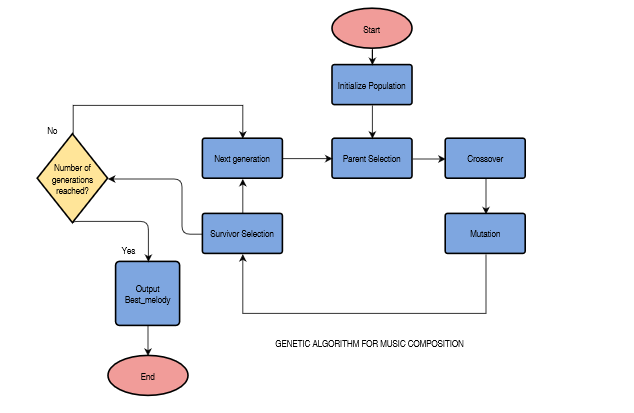
\includegraphics[width=10 cm, height= 10 cm ]{Flowchart.png}
\caption{ Flowchart of the Genetic Algorithm for Music Composition}
\end{figure}

\subsection{Crossover}
Crossover scheme for this algorithm involves choosing a random index in the range of the length of the melody. Each crossover leads to exactly 2 children. The first part of offspring 1 is chosen from parent 1 and the second part from parent 2. On the other hand, the first part of offspring 2 is chosen from parent 2 and the second part from parent 1.

\subsection{Mutation}
Mutation scheme for this algorithm works based on a mutation rate. A random number is generated and if it lies within the set mutation rate, the chromosome is mutated. However, the entire chromosome is not changed. For every beat in the chromosome, a random number is generated and if it is less than the mutation rate, a new beat will be produced.

\subsection{Evolutionary Algorithm}
Combining all techniques above, we evolved the population to find the melody with the highest fitness. At the end of the set $n$ generations, the population is sorted with respect to fitness and the highest fitness melody is stored as the best melody. However, listening to the music allowed us to judge how good the melody is based on how good it sounds to the human ear. Although our algorithm was not an "interactive composition" algorithm, this allowed us to adjust the multipliers for the fitness function to produce better music. This was done during the experimentation process to find the best combination of paramters and fitness multipliers.

\subsection{Generating Music Files Using PySynth}
We used a library ``PySynth B" to produce music files. The chromosome structure is treated such that the melody is turned into a ``.wav" file which is playable by any music player. Its method ``make\_wav" takes a tuple of 2-tuples that describe the melody. The first value of the 2-tuple describes the note and its octave, and the second value describes the duration of the beat. Hence, for PySynth B, the 2-tuple (`c5', 4) denotes a $C5$ beat that plays for a quarter of a second.


\section{Experiment and Results}
%How we tested\\
%What benchmarks we used to evaluate results\\
%Dataset used\\
%Experiment settings\\
%Results and comparison if done\\
%Analysis of results (whether they are good; if they are bad, then in what situations are they bad)\\
We tested our algorithm with different sets of parameters. Controlling population size, mutation rate , selection schemes, offspring size and number of generations, we tried to produce harmonious melodies. As expected, human interaction was necessary to identify good pieces of melody. At each moment that we made a change in parameters, we would stop and listen to the best melody generated at the end to judge how well the algorithm is working.

After experimentation with different parameter values, we set the following parameters:
\begin{align*}
\text{Population size}=50\\
\text{Mutation rate} = 0.6\\
\text{Selection rate} = 0.8\\
\text{Offspring size}= 10\\
\text{Generations}= 5000\\
\end{align*}

We started with a low mutation rate, offspring size and generations and only using the truncation selection scheme, but the fitness value of the population did not change too much and the melody produced at the end wasn't too pleasing to hear. We tweaked these parameters until the melody at the end was much better. We used the binary tournament selection scheme to select the parents and truncation for only selecting the new generation, and our results vastly improved.

\section{Conclusion}
The study was limited by human interaction. We were bound to listen to the music besides simply trusting the fitness function. This breaks complete dependence on the computer for generating music and involves the human brain to pass judgment. A melodious tune may not be rightly identified by the genetic algorithm, but we have gotten close to achieving a harmonious melody at the end of our study. Since we have built up on other works on this topic, we believe that a mathematician who has worked deeply on music's relation to mathematics can help find a better fitness function. There is room for improvement in this search and we believe it is possible to remove human dependence in the innovative and creative task of music composition.

\section*{Acknowledgment}
We thank Dr. Syeda Saleha Raza for teaching us the course \textit{Computational Intelligence} which have allowed us to explore in depth the concept of genetic algorithms and study applications of it. We thank the researchers who have studied this topic deeply and provided us with papers that have increased our knowledge of the subject. We thank other online resources that have facilitated us to understand music terminologies, We thank our lovely friend, Faiza Amir who helped us understand musical terms because of her great interest in composing music.


\begin{thebibliography}{00}
\bibitem{b1} D. Matic, ``A genetic algorithm for composing music," \textit{Yugoslav Journal of Operations Research}, vol. 20, no. 1, pp. 157-177, 2010. Available: 10.2298/yjor1001157m [Accessed 19 April 2019].
\bibitem{b2}V. Anderling, O. Andreasson, C. Olsson, S. Pavlov, C. Svensson, and J. Wikner, ``Generation of music through genetic algorithms," 2014.
\bibitem{b3}G. Papadopoulos and G. Wiggins, ``A Genetic Algorithm for the Generation of Jazz Melodies," 2000
\end{thebibliography}

\end{document}
